% TODO checklist:
% - [x] README.md: Domain entities overview, project structure
% - [x] Q&A.md (Section A, Q4-Q6): Domain entities, agent run lifecycle, job lifecycle
% - [x] Q&A.md (Section F, Q36-Q38): Agent run structure, MCP tools, jobs framework
% - [x] db/postgres_control/models/: SQLAlchemy ORM definitions
% - [x] src/schemas/: Pydantic schema definitions

\section{Domain Model and Core Concepts}
\label{sec:domain-model}

This section defines the core domain entities and their relationships within the Cineca Agentic Platform. Understanding these concepts is essential for comprehending the system's behavior, data flows, and architectural decisions. The domain model reflects enterprise requirements including multi-tenancy, auditability, and extensibility.

\subsection{Entity Overview}

The platform's domain model comprises ten primary entity categories, organized hierarchically from organizational context to operational artifacts. Figure~\ref{fig:domain-model} illustrates the relationships between these entities.

\begin{figure}[htbp]
    \centering
    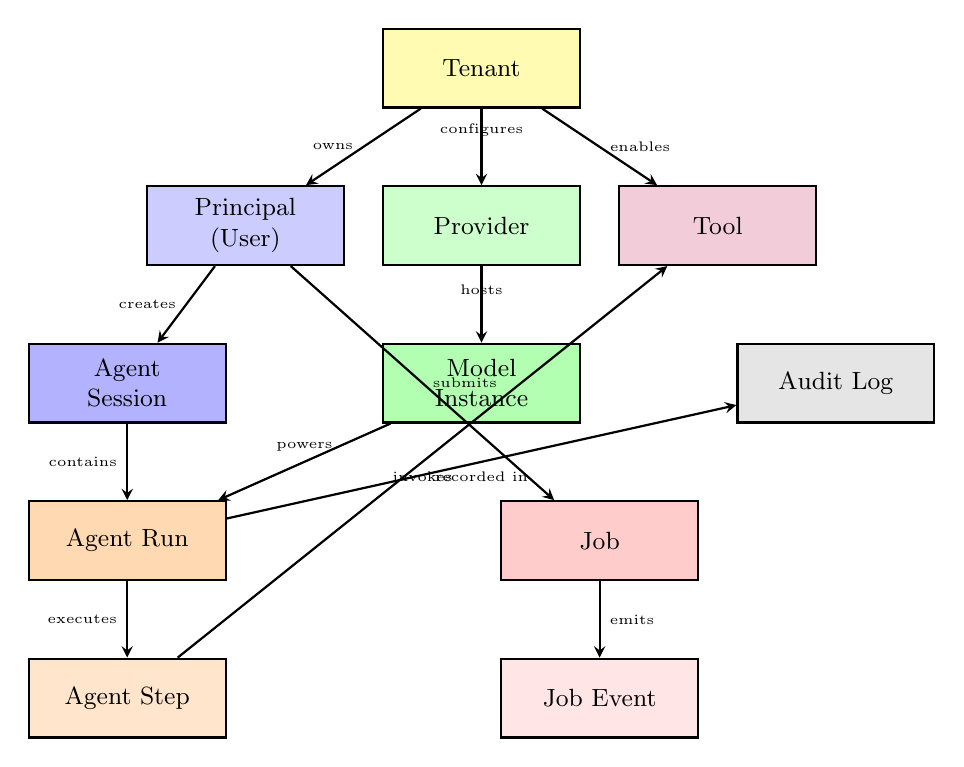
\begin{tikzpicture}[
        node distance=1.5cm,
        entity/.style={rectangle, draw=black, thick, minimum width=2.5cm, minimum height=1cm, align=center, font=\small},
        relation/.style={->, thick, >=stealth},
        label/.style={font=\tiny, midway, above}
    ]
        % Top level - Tenant
        \node[entity, fill=yellow!30] (tenant) at (0, 5) {Tenant};
        
        % Second level - Principal and Provider
        \node[entity, fill=blue!20] (principal) at (-3, 3) {Principal\\(User)};
        \node[entity, fill=green!20] (provider) at (0, 3) {Provider};
        \node[entity, fill=purple!20] (tool) at (3, 3) {Tool};
        
        % Third level - Session and Model
        \node[entity, fill=blue!30] (session) at (-4.5, 1) {Agent\\Session};
        \node[entity, fill=green!30] (model) at (0, 1) {Model\\Instance};
        
        % Fourth level - Runs and Jobs
        \node[entity, fill=orange!30] (run) at (-4.5, -1) {Agent Run};
        \node[entity, fill=red!20] (job) at (1.5, -1) {Job};
        
        % Fifth level - Steps and Events
        \node[entity, fill=orange!20] (step) at (-4.5, -3) {Agent Step};
        \node[entity, fill=red!10] (event) at (1.5, -3) {Job Event};
        
        % Audit (side)
        \node[entity, fill=gray!20] (audit) at (4.5, 1) {Audit Log};
        
        % Relationships
        \draw[relation] (tenant) -- node[label, left] {owns} (principal);
        \draw[relation] (tenant) -- node[label] {configures} (provider);
        \draw[relation] (tenant) -- node[label, right] {enables} (tool);
        \draw[relation] (principal) -- node[label, left] {creates} (session);
        \draw[relation] (provider) -- node[label] {hosts} (model);
        \draw[relation] (session) -- node[label, left] {contains} (run);
        \draw[relation] (run) -- node[label, left] {executes} (step);
        \draw[relation] (model) -- node[label] {powers} (run);
        \draw[relation] (principal) -- node[label, right] {submits} (job);
        \draw[relation] (job) -- node[label, right] {emits} (event);
        \draw[relation] (run) -- node[label, below] {recorded in} (audit);
        \draw[relation] (step) -- node[label, below] {invokes} (tool);
    \end{tikzpicture}
    \caption{Domain model showing primary entities and their relationships.}
    \label{fig:domain-model}
\end{figure}

\subsection{Tenant}

A \textbf{Tenant} represents an organizational boundary for resource isolation and access control. In the CINECA context, tenants correspond to research institutions, departments, or project groups that share the platform infrastructure while maintaining data separation.

\paragraph{Key Attributes}
\begin{itemize}
    \item \texttt{id}: UUID primary key
    \item \texttt{name}: Human-readable tenant name
    \item \texttt{slug}: URL-safe identifier for routing
    \item \texttt{config\_json}: Tenant-specific configuration overrides (JSONB)
    \item \texttt{enabled}: Boolean flag for tenant activation
    \item \texttt{created\_at}, \texttt{updated\_at}: Timestamps for lifecycle tracking
\end{itemize}

\paragraph{Tenant Isolation}
All user-facing data includes a \texttt{tenant\_id} foreign key, enforced through:
\begin{enumerate}
    \item \textbf{Middleware}: Extracts tenant context from \texttt{X-Tenant-ID} header or JWT claims
    \item \textbf{Repository Layer}: Automatically scopes queries to the current tenant
    \item \textbf{Database Constraints}: Foreign key relationships prevent cross-tenant data access
\end{enumerate}

\subsection{Principal}

A \textbf{Principal} represents an authenticated identity---either a human user or a machine client---that can perform actions within the platform. Principals are identified by their \texttt{sub} (subject) claim from the OIDC identity provider.

\paragraph{Principal Types}
\begin{itemize}
    \item \textbf{User}: Human operator authenticated via Auth0 password realm
    \item \textbf{Admin}: User with elevated privileges (e.g., \texttt{admin:all} scope)
    \item \textbf{Machine}: Service account using client credentials flow
\end{itemize}

\paragraph{Key Attributes}
\begin{itemize}
    \item \texttt{sub}: OIDC subject identifier (primary key)
    \item \texttt{email}: Optional email address
    \item \texttt{roles}: Array of assigned roles
    \item \texttt{scopes}: Array of granted OAuth2 scopes
    \item \texttt{tenant\_id}: Associated tenant context
\end{itemize}

\subsection{LLM Provider and Model Instance}

The platform decouples LLM configuration into two entities to enable flexible multi-model deployments.

\paragraph{Provider}
A \textbf{Provider} represents an LLM backend service (e.g., OpenAI API, Ollama server, Azure OpenAI). Key attributes include:
\begin{itemize}
    \item \texttt{id}: UUID primary key
    \item \texttt{name}: Provider identifier (e.g., ``openai'', ``ollama'')
    \item \texttt{api\_type}: API protocol (``openai'', ``azure'', ``ollama'')
    \item \texttt{base\_url}: Endpoint URL for API calls
    \item \texttt{api\_key}: Encrypted credential (nullable for local providers)
    \item \texttt{enabled}: Activation status
    \item \texttt{tenant\_id}: Owning tenant (nullable for global providers)
\end{itemize}

\paragraph{Model Instance}
A \textbf{Model Instance} represents a specific model deployment on a provider. This two-level hierarchy allows multiple instances of the same model with different configurations:
\begin{itemize}
    \item \texttt{id}: UUID primary key
    \item \texttt{instance\_name}: Human-readable name (e.g., ``gpt-4-turbo-prod'')
    \item \texttt{model\_name}: Underlying model identifier (e.g., ``gpt-4-turbo-preview'')
    \item \texttt{provider\_id}: Foreign key to provider
    \item \texttt{temperature}: Default sampling temperature
    \item \texttt{max\_tokens}: Token limit for responses
    \item \texttt{loaded}: Whether model is ready for inference
    \item \texttt{enabled}: Activation status
\end{itemize}

\subsection{Agent Session and Run}

Agent execution is organized into sessions containing multiple runs, enabling conversation continuity and context management.

\paragraph{Agent Session}
An \textbf{Agent Session} groups related agent interactions, providing:
\begin{itemize}
    \item \texttt{id}: UUID primary key
    \item \texttt{owner\_sub}: Principal who created the session
    \item \texttt{tenant\_id}: Tenant context
    \item \texttt{title}: Optional session title
    \item \texttt{context\_json}: Shared context across runs (JSONB)
    \item \texttt{created\_at}, \texttt{expires\_at}: Session lifecycle
\end{itemize}

\paragraph{Agent Run}
An \textbf{Agent Run} represents a single orchestration execution triggered by a user prompt. Key attributes include:
\begin{itemize}
    \item \texttt{id}: UUID primary key
    \item \texttt{session\_id}: Parent session (nullable for standalone runs)
    \item \texttt{status}: Current state (queued, planning, running, succeeded, failed, cancelled)
    \item \texttt{prompt}: User input that initiated the run
    \item \texttt{final\_answer}: Agent's response upon completion
    \item \texttt{model\_instance\_id}: LLM used for orchestration
    \item \texttt{started\_at}, \texttt{finished\_at}: Execution timestamps
    \item \texttt{total\_tokens}, \texttt{llm\_cost\_usd}: Usage metrics
    \item \texttt{todos\_json}: Planned tasks (JSONB)
    \item \texttt{metadata\_json}: Additional execution metadata
\end{itemize}

\paragraph{Agent Step}
Each run comprises multiple \textbf{Agent Steps} representing individual reasoning or action cycles:
\begin{itemize}
    \item \texttt{id}: UUID primary key
    \item \texttt{run\_id}: Parent run
    \item \texttt{step\_number}: Sequential index within run
    \item \texttt{action}: Step type (``think'', ``tool\_call'', ``answer'')
    \item \texttt{tool\_name}: Tool invoked (nullable)
    \item \texttt{tool\_input\_json}: Tool parameters (JSONB)
    \item \texttt{tool\_output\_json}: Tool result (JSONB)
    \item \texttt{reasoning}: LLM's reasoning text
    \item \texttt{duration\_ms}: Step execution time
    \item \texttt{tokens\_used}: Token consumption
\end{itemize}

\subsection{MCP Tool}

An \textbf{MCP Tool} (Model Context Protocol Tool) represents a capability that agents can invoke during execution. Unlike other entities, tools are defined in code rather than the database, with metadata exposed through discovery endpoints.

\paragraph{Tool Metadata}
\begin{itemize}
    \item \texttt{name}: Qualified name (e.g., ``graph.query'', ``jobs.create'')
    \item \texttt{description}: Human-readable purpose
    \item \texttt{schema}: JSON Schema for input validation
    \item \texttt{capabilities}: Feature flags (e.g., ``writes\_db'', ``external\_api'')
    \item \texttt{required\_scopes}: OAuth2 scopes needed for invocation
    \item \texttt{timeout\_ms}: Maximum execution time
    \item \texttt{category}: Organizational grouping
\end{itemize}

\paragraph{Tool Categories}
The platform provides 34 tools organized into 17 categories:
\begin{itemize}
    \item \textbf{Graph}: Cypher query, NL-to-Cypher, schema introspection
    \item \textbf{Jobs}: Creation, status, cancellation
    \item \textbf{Files}: Read, write, list operations
    \item \textbf{Models}: Provider and instance management
    \item \textbf{Admin}: Tenant operations, system configuration
    \item \textbf{Utility}: Date/time, formatting, validation
\end{itemize}

\subsection{Job and Job Event}

The \textbf{Job} entity represents asynchronous background work that executes independently of HTTP request lifecycles.

\paragraph{Job Attributes}
\begin{itemize}
    \item \texttt{id}: UUID primary key
    \item \texttt{type}: Job classification (e.g., ``batch\_export'', ``graph\_sync'')
    \item \texttt{status}: Current state (queued, running, finished, failed, cancelled)
    \item \texttt{owner\_sub}: Submitting principal
    \item \texttt{tenant\_id}: Tenant context
    \item \texttt{payload\_json}: Input parameters (JSONB)
    \item \texttt{result\_json}: Output data (JSONB)
    \item \texttt{error}: Failure message (nullable)
    \item \texttt{priority}: Queue ordering (0 = normal, higher = more urgent)
    \item \texttt{idempotency\_key}: For duplicate detection
    \item \texttt{created\_at}, \texttt{started\_at}, \texttt{completed\_at}: Lifecycle timestamps
\end{itemize}

\paragraph{Job Events}
\textbf{Job Events} provide an append-only log of job state changes and progress updates:
\begin{itemize}
    \item \texttt{seq\_id}: Monotonic sequence number (primary key)
    \item \texttt{job\_id}: Parent job
    \item \texttt{event\_type}: Category (``status'', ``log'', ``progress'', ``heartbeat'', ``end'')
    \item \texttt{event\_json}: Event payload (JSONB)
    \item \texttt{created\_at}: Event timestamp
\end{itemize}

Events are streamed to clients via Server-Sent Events (SSE), enabling real-time progress monitoring without polling.

\subsection{Audit Log}

The \textbf{Audit Log} provides an immutable record of security-relevant actions for compliance and forensics.

\paragraph{Audit Entry Attributes}
\begin{itemize}
    \item \texttt{id}: UUID primary key
    \item \texttt{timestamp}: Event time (with timezone)
    \item \texttt{actor\_sub}: Principal performing the action
    \item \texttt{tenant\_id}: Tenant context
    \item \texttt{action}: Operation type (e.g., ``agent.run.create'', ``tool.invoke'')
    \item \texttt{resource\_type}: Entity type affected
    \item \texttt{resource\_id}: Entity identifier
    \item \texttt{details\_json}: Additional context (JSONB)
    \item \texttt{outcome}: Success or failure indicator
    \item \texttt{client\_ip}: Source IP address
    \item \texttt{request\_id}: Correlation identifier
\end{itemize}

\subsection{Entity Lifecycle Summary}

Table~\ref{tab:entity-lifecycle} summarizes the state machines governing primary entity lifecycles.

\begin{table}[htbp]
    \centering
    \caption{State transitions for primary domain entities.}
    \label{tab:entity-lifecycle}
    \small
    \begin{tabular}{lll}
        \toprule
        \textbf{Entity} & \textbf{States} & \textbf{Terminal States} \\
        \midrule
        Agent Run & queued $\to$ planning $\to$ running & succeeded, failed, cancelled \\
        Job & queued $\to$ running & finished, failed, cancelled \\
        Session & active $\to$ expired & expired, archived \\
        Provider & enabled, disabled & (soft delete) \\
        Model Instance & loading $\to$ loaded, unloaded & (soft delete) \\
        \bottomrule
    \end{tabular}
\end{table}

\subsection{Glossary of Terms}

For reference, Table~\ref{tab:domain-glossary} provides concise definitions of key domain terminology used throughout this thesis.

\begin{table}[htbp]
    \centering
    \caption{Glossary of domain terminology.}
    \label{tab:domain-glossary}
    \small
    \begin{tabularx}{\textwidth}{lX}
        \toprule
        \textbf{Term} & \textbf{Definition} \\
        \midrule
        Tenant & Organizational unit for resource isolation and access control \\
        Principal & Authenticated identity (user or machine) with assigned permissions \\
        Provider & LLM backend service hosting one or more model instances \\
        Model Instance & Specific model deployment with configuration parameters \\
        Agent Session & Container for related agent runs enabling conversation continuity \\
        Agent Run & Single orchestration execution from prompt to final answer \\
        Agent Step & Individual reasoning or action cycle within a run \\
        MCP Tool & Capability that agents can invoke during execution \\
        Job & Asynchronous background work independent of HTTP requests \\
        Audit Log & Immutable record of security-relevant actions \\
        Scope & OAuth2 permission grant (e.g., \texttt{tools:invoke:basic}) \\
        RBAC & Role-Based Access Control for authorization decisions \\
        \bottomrule
    \end{tabularx}
\end{table}
